\section{Definição de Função}

\begin{definition}
Sejam $X$ e $Y$ dois conjuntos quaisquer.
Uma \textdef{função} é uma relação $f: X \to Y$ (lê-se $f$ de $X$ em $Y$) que, a cada elemento $x \in X$, associa um e somente um elemento $y \in Y$.
Definem-se, além disso, os seguintes termos:
%
\begin{enumerate}[(i)]
\item \textdef{Domínio} e \textdef{contradomínio} de $f$ para os conjuntos $X$ e $Y$, respectivamente;
\item \textdef{Imagem} de $x$, dado $x \in X$, para o único elemento $y \in Y$ que satisfaz $y = f(x)$;
\item \textdef{Imagem} de $f$ para o conjunto $f\prn X = \set{y \in Y \tq y = f \prn x \text{ para algum } x \in X }$, ou seja, o conjunto de todas as \emph{imagens} de $x$ para todo $x \in X$.

Confira o exemplo a seguir:
\begin{center}
    \tikzset{every picture/.style={line width=0.75pt}} %set default line width to 0.75pt        

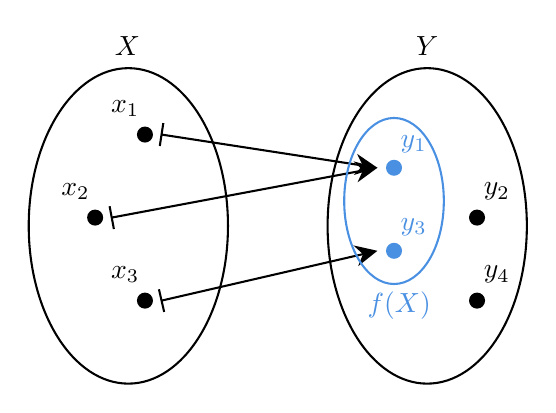
\begin{tikzpicture}[x=0.75pt,y=0.75pt,yscale=-1,xscale=1]
%uncomment if require: \path (0,308); %set diagram left start at 0, and has height of 308

%Shape: Ellipse [id:dp8584080168945698] 
\draw   (160,124) .. controls (160,82.03) and (181.49,48) .. (208,48) .. controls (234.51,48) and (256,82.03) .. (256,124) .. controls (256,165.97) and (234.51,200) .. (208,200) .. controls (181.49,200) and (160,165.97) .. (160,124) -- cycle ;
%Straight Lines [id:da9209150729175881] 
\draw    (216,80) ;

\draw [shift={(216,80)}, rotate = 0] [color={rgb, 255:red, 0; green, 0; blue, 0 }  ][fill={rgb, 255:red, 0; green, 0; blue, 0 }  ][line width=0.75]      (0, 0) circle [x radius= 3.35, y radius= 3.35]   ;
%Straight Lines [id:da7784202535308219] 
\draw [color={rgb, 255:red, 74; green, 144; blue, 226 }  ,draw opacity=1 ]   (336,96) ;

\draw [shift={(336,96)}, rotate = 0] [color={rgb, 255:red, 74; green, 144; blue, 226 }  ,draw opacity=1 ][fill={rgb, 255:red, 74; green, 144; blue, 226 }  ,fill opacity=1 ][line width=0.75]      (0, 0) circle [x radius= 3.35, y radius= 3.35]   ;
%Shape: Ellipse [id:dp3856498056795209] 
\draw   (304,124) .. controls (304,82.03) and (325.49,48) .. (352,48) .. controls (378.51,48) and (400,82.03) .. (400,124) .. controls (400,165.97) and (378.51,200) .. (352,200) .. controls (325.49,200) and (304,165.97) .. (304,124) -- cycle ;
%Straight Lines [id:da4011502733578831] 
\draw    (200,120) -- (326.03,96.37) ;
\draw [shift={(328,96)}, rotate = 529.38] [fill={rgb, 255:red, 0; green, 0; blue, 0 }  ][line width=0.75]  [draw opacity=0] (10.72,-5.15) -- (0,0) -- (10.72,5.15) -- (7.12,0) -- cycle    ;
\draw [shift={(200,120)}, rotate = 529.38] [color={rgb, 255:red, 0; green, 0; blue, 0 }  ][line width=0.75]    (0,5.59) -- (0,-5.59)   ;
%Straight Lines [id:da7099724823991076] 
\draw [color={rgb, 255:red, 74; green, 144; blue, 226 }  ,draw opacity=1 ]   (336,136) ;

\draw [shift={(336,136)}, rotate = 0] [color={rgb, 255:red, 74; green, 144; blue, 226 }  ,draw opacity=1 ][fill={rgb, 255:red, 74; green, 144; blue, 226 }  ,fill opacity=1 ][line width=0.75]      (0, 0) circle [x radius= 3.35, y radius= 3.35]   ;
%Straight Lines [id:da4810899906621904] 
\draw    (192,120) ;

\draw [shift={(192,120)}, rotate = 0] [color={rgb, 255:red, 0; green, 0; blue, 0 }  ][fill={rgb, 255:red, 0; green, 0; blue, 0 }  ][line width=0.75]      (0, 0) circle [x radius= 3.35, y radius= 3.35]   ;
%Straight Lines [id:da1387493271002489] 
\draw    (216,160) ;

\draw [shift={(216,160)}, rotate = 0] [color={rgb, 255:red, 0; green, 0; blue, 0 }  ][fill={rgb, 255:red, 0; green, 0; blue, 0 }  ][line width=0.75]      (0, 0) circle [x radius= 3.35, y radius= 3.35]   ;
%Straight Lines [id:da07664909250691976] 
\draw    (376,120) ;

\draw [shift={(376,120)}, rotate = 0] [color={rgb, 255:red, 0; green, 0; blue, 0 }  ][fill={rgb, 255:red, 0; green, 0; blue, 0 }  ][line width=0.75]      (0, 0) circle [x radius= 3.35, y radius= 3.35]   ;
%Straight Lines [id:da9651324228114074] 
\draw    (376,160) ;

\draw [shift={(376,160)}, rotate = 0] [color={rgb, 255:red, 0; green, 0; blue, 0 }  ][fill={rgb, 255:red, 0; green, 0; blue, 0 }  ][line width=0.75]      (0, 0) circle [x radius= 3.35, y radius= 3.35]   ;
%Straight Lines [id:da7557341854466749] 
\draw    (224,160) -- (326.05,136.45) ;
\draw [shift={(328,136)}, rotate = 527.01] [fill={rgb, 255:red, 0; green, 0; blue, 0 }  ][line width=0.75]  [draw opacity=0] (10.72,-5.15) -- (0,0) -- (10.72,5.15) -- (7.12,0) -- cycle    ;
\draw [shift={(224,160)}, rotate = 527.01] [color={rgb, 255:red, 0; green, 0; blue, 0 }  ][line width=0.75]    (0,5.59) -- (0,-5.59)   ;
%Straight Lines [id:da17659401986386492] 
\draw    (224,80) -- (326.02,95.7) ;
\draw [shift={(328,96)}, rotate = 188.75] [fill={rgb, 255:red, 0; green, 0; blue, 0 }  ][line width=0.75]  [draw opacity=0] (10.72,-5.15) -- (0,0) -- (10.72,5.15) -- (7.12,0) -- cycle    ;
\draw [shift={(224,80)}, rotate = 188.75] [color={rgb, 255:red, 0; green, 0; blue, 0 }  ][line width=0.75]    (0,5.59) -- (0,-5.59)   ;
%Shape: Ellipse [id:dp8087351065679074] 
\draw  [color={rgb, 255:red, 74; green, 144; blue, 226 }  ,draw opacity=1 ] (312,112) .. controls (312,89.91) and (322.75,72) .. (336,72) .. controls (349.25,72) and (360,89.91) .. (360,112) .. controls (360,134.09) and (349.25,152) .. (336,152) .. controls (322.75,152) and (312,134.09) .. (312,112) -- cycle ;

% Text Node
\draw (207.5,37.5) node   {$X$};
% Text Node
\draw (352,37.5) node   {$Y$};
% Text Node
\draw (338.5,162.5) node [color={rgb, 255:red, 74; green, 144; blue, 226 }  ,opacity=1 ]  {$f( X)$};
% Text Node
\draw (206.5,67.5) node   {$x_{1}$};
% Text Node
\draw (182.5,107.5) node   {$x_{2}$};
% Text Node
\draw (206.5,147.5) node   {$x_{3}$};
% Text Node
\draw (345.5,84.5) node [color={rgb, 255:red, 74; green, 144; blue, 226 }  ,opacity=1 ]  {$y_{1}$};
% Text Node
\draw (345.5,124.5) node [color={rgb, 255:red, 74; green, 144; blue, 226 }  ,opacity=1 ]  {$y_{3}$};
% Text Node
\draw (385.5,107.5) node [color={rgb, 255:red, 0; green, 0; blue, 0 }  ,opacity=1 ]  {$y_{2}$};
% Text Node
\draw (385.5,147.5) node [color={rgb, 255:red, 0; green, 0; blue, 0 }  ,opacity=1 ]  {$y_{4}$};

\end{tikzpicture}
\end{center}
Observe que o conjunto imagem de $f$, por ser constituído de elementos de $Y$, sempre está contido no contradomínio, isto é, $f(X) \subset Y$.
\end{enumerate}
\end{definition}

%\begin{remark}
%\label{rem:def-alternativa-funcao}
De certa forma, uma função pode ser vista como um terno constituído por: \textdef{domínio}, \textdef{contradomínio} e \textdef{lei de associação} (dos elementos do domínio com os do contradomínio). 
Precisa-se desses três elementos para que uma função seja bem-definida. 

A definição alternativa a seguir também poderia ser adotada:
{\it Uma relação $f: X \to Y$ é uma \emph {função} se satisfaz as seguintes condições:
%
\begin{enumerate}[(I)]
  \item Estar bem-definida em todo elemento do domínio, isto é, os elementos do domínio devem corresponder à pelo menos um elemento do contradomínio;
  \item Os elementos do domínio não devem corresponder a mais de um elemento do contradomínio, ou seja, devem corresponder no máximo um elemento.
\end{enumerate}}
%\end{remark}


\begin{example}
Sejam $X = \set{x_1, x_2}$ e $Y = \set{y_1, y_2}$ e a relação $f : X \to Y$ definida pelo gráfico a seguir:
\begin{center}
     
\tikzset{every picture/.style={line width=0.75pt}} %set default line width to 0.75pt        

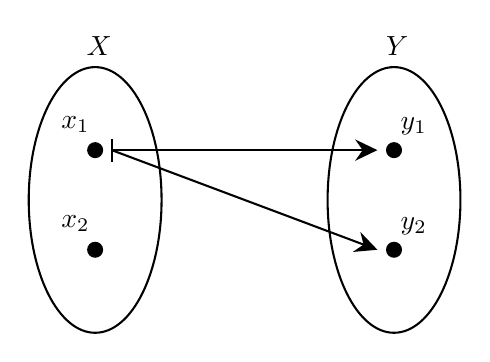
\begin{tikzpicture}[x=0.75pt,y=0.75pt,yscale=-1,xscale=1]
%uncomment if require: \path (0,308); %set diagram left start at 0, and has height of 308

%Shape: Ellipse [id:dp8584080168945698] 
\draw   (160,112) .. controls (160,76.65) and (174.33,48) .. (192,48) .. controls (209.67,48) and (224,76.65) .. (224,112) .. controls (224,147.35) and (209.67,176) .. (192,176) .. controls (174.33,176) and (160,147.35) .. (160,112) -- cycle ;
%Straight Lines [id:da9209150729175881] 
\draw    (192,88) ;

\draw [shift={(192,88)}, rotate = 0] [color={rgb, 255:red, 0; green, 0; blue, 0 }  ][fill={rgb, 255:red, 0; green, 0; blue, 0 }  ][line width=0.75]      (0, 0) circle [x radius= 3.35, y radius= 3.35]   ;
%Straight Lines [id:da7784202535308219] 
\draw    (336,88) ;

\draw [shift={(336,88)}, rotate = 0] [color={rgb, 255:red, 0; green, 0; blue, 0 }  ][fill={rgb, 255:red, 0; green, 0; blue, 0 }  ][line width=0.75]      (0, 0) circle [x radius= 3.35, y radius= 3.35]   ;
%Shape: Ellipse [id:dp3856498056795209] 
\draw   (304,112) .. controls (304,76.65) and (318.33,48) .. (336,48) .. controls (353.67,48) and (368,76.65) .. (368,112) .. controls (368,147.35) and (353.67,176) .. (336,176) .. controls (318.33,176) and (304,147.35) .. (304,112) -- cycle ;
%Straight Lines [id:da4011502733578831] 
\draw    (200,88) -- (326,88) ;
\draw [shift={(328,88)}, rotate = 180] [fill={rgb, 255:red, 0; green, 0; blue, 0 }  ][line width=0.75]  [draw opacity=0] (10.72,-5.15) -- (0,0) -- (10.72,5.15) -- (7.12,0) -- cycle    ;
\draw [shift={(200,88)}, rotate = 180] [color={rgb, 255:red, 0; green, 0; blue, 0 }  ][line width=0.75]    (0,5.59) -- (0,-5.59)   ;
%Straight Lines [id:da7099724823991076] 
\draw    (336,136) ;

\draw [shift={(336,136)}, rotate = 0] [color={rgb, 255:red, 0; green, 0; blue, 0 }  ][fill={rgb, 255:red, 0; green, 0; blue, 0 }  ][line width=0.75]      (0, 0) circle [x radius= 3.35, y radius= 3.35]   ;
%Straight Lines [id:da6485112628479169] 
\draw    (192,136) ;

\draw [shift={(192,136)}, rotate = 0] [color={rgb, 255:red, 0; green, 0; blue, 0 }  ][fill={rgb, 255:red, 0; green, 0; blue, 0 }  ][line width=0.75]      (0, 0) circle [x radius= 3.35, y radius= 3.35]   ;
%Straight Lines [id:da9851163463272556] 
\draw    (200,88) -- (326.13,135.3) ;
\draw [shift={(328,136)}, rotate = 200.56] [fill={rgb, 255:red, 0; green, 0; blue, 0 }  ][line width=0.75]  [draw opacity=0] (10.72,-5.15) -- (0,0) -- (10.72,5.15) -- (7.12,0) -- cycle    ;


% Text Node
\draw (182.5,75.5) node   {$x_{1}$};
% Text Node
\draw (194,38) node   {$X$};
% Text Node
\draw (337.5,38) node   {$Y$};
% Text Node
\draw (345.5,76.5) node   {$y_{1}$};
% Text Node
\draw (345.5,124.5) node   {$y_{2}$};
% Text Node
\draw (182.5,123.5) node   {$x_{2}$};


\end{tikzpicture}
\end{center}
Qual(is) o(s) problema(s) com essa ``função''?
\end{example}
\begin{solution}
Temos dois problemas, o primeiro é que, pelo gráfico, temos que $f(x_1) = y_1$ e $f(x_1) = y_2$, e com isso existem dois valores possíveis para $f(x_1)$. O segundo é que $x_2$ não foi mapeado em nenhum elemento de $Y$, sendo assim não há um valor para $f(x_2)$.
\end{solution}


\begin{example}
\label{example:func-sq-sqrt}
Considere as funções $p$ e $q$ a seguir:
%
\begin{gather*}
\begin{array}{cccc}
p : & \R & \to     & \R_+ \\
     &  x & \mapsto & x^2;
\end{array}\\
\begin{array}{cccc}
q : & \R_+ & \to     & \R \\
     &  x & \mapsto & \sqrt x
\end{array}.
\end{gather*}
%
Qual o domínio, contradomínio e a lei de associação de $p$ e $q$?
\end{example}

\begin{solution}
O domínio de $p$ é $\R$ e o de $q$ é $\R_+$; 
O contradomínio de $p$ é $\R_+$ e o de $q$ é $\R$; 
A lei de associação de $p$ é $p(x)=x^2$ e a de $q$ é $q(x)=\sqrt x$.
\end{solution}

\begin{definition}
Seja $\identity X : X \to X $ uma função tal que $\identity X \prn x = x$ para todo $x \in X$. Chamamos $\identity X$ de \textdef{função identidade do conjunto $X$}.
\end{definition}